\chapter{Výsledky práce}
Medzi najdôležitejšie tu nachádzajúce sa dielo patria problémové úlohy z programovania pre začiatočníkov na stredných školách. V súvislosti s našou zbierkou úloh rozoberieme adoptovanú anatómiu úlohy a dôsledky vyplývajúce z terajšieho zoradenia cvičení. Vychádzame pritom z teoretických základov tvorby učebníc a požiadaviek na pestrosť aplikáčného prostredia pre pojmy za účelom pritiahnutia záujmu učiaceho sa subjektu.

\section{Zbierka úloh}
Zhromaždený súbor zadaní z programovania sa skladá počtom z 54 úloh s riešeniami, ktoré sú rozčlenené do tématických častí nerovnomerne. Oddiel premenné má 11 úloh, podmienky - 9 úloh, cykly - 9 úloh, náhodné čísla - 3 úlohy, reťazce a zoznamy - 9 úloh, súbory - 5 úloh, funkcie - 8 úloh. Usporiadanie celkov teda pochádza čiastočne zo vzdelávacích štandardov ale aj zvyklostí.

Nepravidelnosti v kvantite častí nastali kvôli organickému a postupnému pribúdaniu úloh, ktoré reagovalo na potreby žiakov vedúce k zvládnutiu predmetu. Na kostru úloh sa dodatočne nabalili aj niektoré testové problémy, cvičenia na doma, ale upravene i učivo z iných predmetov, ktoré trápilo žiakov pred písomkami. K zdanlivo relatívne menšiemu objemu časti súbory poznamenáme, že v skutočnosti prvá úloha spočíva v prispôsobeniu všetkých úloh z predošlej témy na súbory. Prísne vzaté na súbory je preto k dispozícii až 13 úloh.

Podľa didaktickej zásady spojenia teórie s praxov a na prispenie ku kompentencii celoživotného učenia sa pre život dbáme na interdisciplinaritu nastolených problémov zasadených do reálneho sveta. Medzipredmetové aplikácie čerpajú z matematiky (16 úloh) a finančnej gramotnosti (2 úlohy), fyziky (4 úlohy), slovenského jazyka a literatúry (3 úlohy), geografie (2 úlohy), dejepisu (2 úlohy) a chémie (1 úloha). 

Matematika má z hľadiska využitia jej aparátu v programátorských úlohách nespornú výhodu pre blízkosť k informatike ako takej. Existujú zároveň viaceré možnosti znovupoužitia príkladov z matematických učebníc. K medzipremetovým vzťahov s \textbf{matematikou} prispievajú témy:
\begin{itemize}[noitemsep,topsep=0pt]
\item objem a obsah telies \emph{(1.6, 1.8, 1.9)}
\item meranie času \emph{(2.5)}
\item kalkulačky \emph{(2.6, 7.10)}
\item kvadratické rovnice \emph{(2.8)}
\item trojuholníky \emph{(2.9.)}
\item malá násobilka \emph{(3.8, 4.3)}
\item zlomky a percentá \emph{(5.5, 5.6, 7.6)}
\item finančná gramotnosť \emph{(3.9, 5.7)}
\item súradnicová sústava \emph{(7.1)}
\item binomická veta \emph{(7.3)}
\item štatistika \emph{(7.4)}
\end{itemize}
Do \textbf{fyziky} môžeme zaradiť úlohy ohľadom: 
\begin{itemize}[noitemsep,topsep=0pt]
\item teploty \emph{(1.4)}
\item kinematiky \emph{(1.5, 1.7)}
\item dynamiky \emph{(1.9)}
\end{itemize}
\textbf{Slovenského jazyka} sa okrajovo týkajú úlohy na:
\begin{itemize}[noitemsep,topsep=0pt]
\item rým \emph{(1.2)}
\item hláskoslovie \emph{(5.2)}
\item tvaroslovie \emph{(5.8)}
\end{itemize}
Pod témy súvisace s \textbf{geografiou} spadajú meteorológia \emph{(2.4)} a kartografia \emph{(6.2)}, z \textbf{chémie} sme zahrnuli roztoky \emph{(1.10)} a z \textbf{dejepisu} sa zmieňujeme o Májskych pyramídach \emph{(3.3)} a rímskych číslach \emph{(7.6)}. 
V zbierke je tiež 9 úloh na rýdzo \textbf{informatické} záležitosti:
\begin{itemize}[noitemsep,topsep=0pt]
\item heslá \emph{(2.1)}
\item hry a simulácie \emph{(4.1, 4.2, 7.7)}
\item šifrovanie \emph{(7.2)}
\item kompresia \emph{(5.9)}
\item databázy \emph{(6.3, 6.4, 6.5)}
\end{itemize}

Výber úloh je aj na učiteľovi, aby pružne reagoval na časové súvislosti v učebných plánoch nadväzujúcic predmetov. Viac nežiadané je predbiehať predmet, z ktorého úloha čerpá, pretože to so sebou nesie znásobené časové nároky na objasnenie a hrozbu nadobudnutia povrchného obrazu o prebratej oblasti z iného vyučovacieho predmetu. Ďalej uvázame znenia zadaní úloh.

\subsection{Premenné}
\underline{\textbf{Premenná}} je taká krabička na odkladanie čísel alebo slov, ktoré si potrebujeme zapamätať na dokončenie činnosti. Premenné sa líšia svojim \underline{\textbf{dátovým typom}}. Premenná dostane svoj typ cez \underline{\textbf{priradenie}}, čiže vtedy keď prvýkrát do nej niečo uložíme. Typ hovorí o tom, čo sa vo vnútri premennej nachádza.

Základné typy premenných sú:
\begin{itemize}[noitemsep,topsep=0pt]
\item \underline{\textbf{Logická hodnota}} (\textit{bool}) - môže mať len dve hodnoty - pravda (\textit{True}) alebo nepravda (\textit{False})
\item \underline{\textbf{Celé číslo}} (\textit{int}) - ukladáme sem ľubovolné kladné a záporné celé čísla (\textit{97})
\item \underline{\textbf{Desatinné číslo}} (\textit{float}) - Líšia sa od celých čísel spôsobom uloženia (\textit{3.14159})
\item \underline{\textbf{Reťazec}} (\textit{str}) - Označujeme ich úvodzovkami alebo apostrofmi a väčšinou predstavujú text napísaný na klávesnici alebo zobrazený na obrazovke \textit{``Učím sa programovať!''}).
\end{itemize}

\subsubsection*{1. Pozdrav}
Skladáš si stavebnicu robotického domáceho miláčika, ktorý je takmer dokonalý. Má telo, končatiny, hlavu a vie kráčať po stole. Keby však sa naučil aj hovoriť, to by bol potom poriadny spoločník. Každý dobrý rozhovor sa začína pozdravom. Napíš program, ktorý ťa pozdraví po napísaní mena na klávesnici. Doplň tiež, aby sa program s tebou aj rozlučil.

\begin{tabular}{@{}p{0.15\linewidth}p{0.75\linewidth}}
\textbf{\small Vstup:} &
\vspace{-3em}
\begin{code}
Ako sa voláš?: @\fbox{\phantom{meno}}@
\end{code}
\end{tabular}

\vspace{-2em}
\begin{tabular}{@{}p{0.15\linewidth}p{0.75\linewidth}}
\textbf{\small Výstup:} &
\vspace{-3em}
\begin{code} 
Ahoj @\fbox{\phantom{meno}}@
\end{code}
\end{tabular}
\vspace{-2em}

\subsubsection*{2. Básnik}
Rozkríklo sa, že píšeš pekné básničky na rôzne príležitosti. Prichádza ti čím ďalej viac prosieb od kamarátov a známych, či im nevytoríš peknú rýmovačku. Vymýšať kreatívne texty je niekedy veľká námaha, tak ti napadne, že stačí meniť len rým. Napíš program, ktorý za teba slovo vloží do predlohy básne.

\begin{tabular}{@{}p{0.15\linewidth}p{0.75\linewidth}}
\textbf{\small Vstup:} &
\vspace{-3em}
\begin{code}
Napíš slovo, ktoré sa rýmuje so slovom strach: @\fbox{\phantom{slovo}}@
\end{code}
\end{tabular}

\vspace{-2em}
\begin{tabular}{@{}p{0.15\linewidth}p{0.75\linewidth}}
\textbf{\small Výstup:} &
\vspace{-3em} 
\begin{code}
Tu je báseň:
Z počítačov mával som vždy strach,
teraz som však šťastný ako @\fbox{\phantom{slovo}}@.
\end{code}
\end{tabular}
\vspace{-2em}

\subsubsection*{3. Pozvánka}
Budúci víkend organizuješ velkolepú narodeninovú párty a rozposielaš na ňu pozvánky. Okrem mena hosťa potrebuješ meniť aj čas konania oslavy. Máš totiž skúsenosti, že nie všetci chodia načas. Každý pozvaný si má priniesť okrem darčeku aj jednu špeciálnu vec. Napíš program, ktorý doplní takúto pozvánku na mieru.

\begin{tabular}{@{}p{0.15\linewidth}p{0.75\linewidth}}
\textbf{\small Vstup:} &
\vspace{-3em}
\begin{code}
Meno kamaráta: @\fbox{\phantom{vstup}}@
Čas oslavy: @\fbox{\phantom{vstup}}@
Prinesie okrem darčeku: @\fbox{\phantom{vstup}}@
\end{code}
\end{tabular}

\vspace{-2em}
\begin{tabular}{@{}p{0.15\linewidth}p{0.75\linewidth}}
\textbf{\small Výstup:} &
\vspace{-3em} 
\begin{code}
Ahoj @\fbox{\phantom{vstup}}@,
pozývam ťa na moju narodeninovú párty.
Bude sa konať 12.4. o @\fbox{\phantom{vstup}}@. 
Nezabudni priniesť @\fbox{\phantom{vstup}}@ a pekný darček.
Teším sa na teba! :)
\end{code}
\end{tabular}
\vspace{-2em}

\subsubsection*{4. Teplota vo Farenheitoch}
Prišiel si na dovolenku do Spojených štátov amerických. Obliekaš sa na krátky výlet von, ale nevieš ako sa máš obliecť. Na teplomeroch sú napísané len stupne Fahrenheita. Napíš program, ktorý ich premení na stupne Celzia s presnosťou na dve desatinné miesta.

\begin{tabular}{@{}p{0.15\linewidth}p{0.75\linewidth}}
\textbf{\small Vstup:} &
\vspace{-3em}
\begin{code}
Vonku je °F: @\fbox{\phantom{vstup}}@
\end{code}
\end{tabular}

\vspace{-2em}
\begin{tabular}{@{}p{0.15\linewidth}p{0.75\linewidth}}
\textbf{\small Výstup:} &
\vspace{-3em} 
\begin{code}
Doma by bolo na teplomeri @\fbox{\phantom{vstup}}@°C.
\end{code}
\end{tabular}
\vspace{-2em}

\subsubsection*{5. Hlboká roklina}
Stojíš nad hlbokým údolím za zábradlím a uvažuješ ako odmerať jeho hĺbku. Vtom si spomenieš na svoje vedomosti z fyziky. Zoberieš si do ruky povaľúci sa kameň a pustíš ho priamo do rokliny. Zároveň stlačíš stopky, ktorými zmeriaš čas do dopadu v sekundách. Kameň padá nadol voľným pádom. Stopky zastaviš pri započutí rachotu z nárazu. Pri výpočte zanedbáme rýchlosť zvuku, ktorou sa rachot rožšíri až k nám.

\begin{tabular}{@{}p{0.15\linewidth}p{0.75\linewidth}}
\textbf{\small Vstup:} &
\vspace{-3em}
\begin{code}
Čas do dopadu kameňa: @\fbox{\phantom{vstup}}@
\end{code}
\end{tabular}

\vspace{-2em}
\begin{tabular}{@{}p{0.15\linewidth}p{0.75\linewidth}}
\textbf{\small Výstup:} &
\vspace{-3em}
\begin{code}
Hĺbka rokliny je @\fbox{\phantom{vstup}}@ metrov.
\end{code}
\end{tabular}
\vspace{-2em}

\subsubsection*{6. Vedro s vodou}
V rodinnom dome ste ekologicky uvedomelí, lebo zachytávate ďaždovú vodu z odkvapu na polievanie záhrady. Minulú noc vám napršalo do nádrže veľa vody. Keď bude o pár dní suchšie mama ťa pošle poliať rastliny uzavretým vedrom valcového tvaru. To naplníš vždy až po okraj. Zaujíma ťa, aký objem naberieš na jedno naplnenie. Rozmery valcového vedra vieš odmerať pravítkom. Napíš program, ktorý zráta koľko sa zmestí vody do rôzne veľkých vedier.

\begin{tabular}{@{}p{0.15\linewidth}p{0.75\linewidth}}
\textbf{\small Vstup:} &
\vspace{-3em}
\begin{code}
Výška vedra (cm): @\fbox{\phantom{vstup}}@
Priemer dna (cm): @\fbox{\phantom{vstup}}@
\end{code}
\end{tabular}

\vspace{-2em}
\begin{tabular}{@{}p{0.15\linewidth}p{0.75\linewidth}}
\textbf{\small Výstup:} &
\vspace{-3em}
\begin{code}
Do vedra sa zmestí @\fbox{\phantom{vstup}}@ litrov vody.
\end{code}
\end{tabular}
\vspace{-2em}

\subsubsection*{7. Cesta autom}
Tešíš sa na očakávaný výlet autom po Európe. Pri plánovaní trasy chceš zistiť akou rýchlosťou musíte priemerne cestovať, aby ste od rána stihli navštíviť všetky miesta. Večer však musíte prísť včas do hotela, aby vás ubytovali. Napíš program, ktorý ti s tým pomôže.

\begin{tabular}{@{}p{0.15\linewidth}p{0.75\linewidth}}
\textbf{\small Vstup:} &
\vspace{-3em}
\begin{code}
Dĺžka cesty (km): @\fbox{\phantom{vstup}}@
Odchod z domu (hodina): @\fbox{\phantom{vstup}}@
Príchod do hotela (hodina): @\fbox{\phantom{vstup}}@
\end{code}
\end{tabular}

\vspace{-2em}
\begin{tabular}{@{}p{0.15\linewidth}p{0.75\linewidth}}
\textbf{\small Výstup:} &
\vspace{-3em}
\begin{code}
Auto pôjde priemernou rýchlosťou @\fbox{\phantom{vstup}}@ km/h.
\end{code}
\end{tabular}
\vspace{-2em}

\subsubsection*{8. Kúpalisko}
Začína sa horúca letná sezóna. Prevádzka kúpaliska musí pred otvorením napustiť bazény. Všetky bazény v areáli sú kvádrového tvaru, ktorých rozmery poznáme. Vedúceho kúpaliska zaujíma spotrebovaná voda pre bazén, keď bude napustený pod okraj. Voda nie je zadarmo, preto si chcú pripraviť dosť peňazí, aby za ňu zaplatili.

\begin{tabular}{@{}p{0.15\linewidth}p{0.75\linewidth}}
\textbf{\small Vstup:} &
\vspace{-3em}
\begin{code}
Dĺžka bazéna (m): @\fbox{\phantom{vstup}}@
Šírka bazéna (m): @\fbox{\phantom{vstup}}@
Hĺbka bazéna (m): @\fbox{\phantom{vstup}}@
Hĺbka hladiny pod okrajom (cm): @\fbox{\phantom{vstup}}@
Cena za m^3 vody v eurách: @\fbox{\phantom{vstup}}@ 
\end{code}
\end{tabular}

\vspace{-2em}
\begin{tabular}{@{}p{0.15\linewidth}p{0.75\linewidth}}
\textbf{\small Výstup:} &
\vspace{-3em}
\begin{code}
Na bazén sa minie @\fbox{\phantom{vstup}}@ litrov vody.
Voda bude stáť @\fbox{\phantom{vstup}}@ eur.
\end{code}
\end{tabular}
\vspace{-2em}

\subsubsection*{9. Maľovanie}
S rodičmi sa sťahuješ do nového bytu. Dali ti za úlohu kúpiť si farbu na vymaľovanie izby. Nástroj na rýchle počítanie množstva farby by sa hodil asi aj profesionálnym maliarom. Vytvor program na vypočítanie plochy stien a stropu bez okna a podlahy.

\begin{tabular}{@{}p{0.15\linewidth}p{0.75\linewidth}}
\textbf{\small Vstup:} &
\vspace{-3em}
\begin{code}
Rozmery miestnosti
Dĺžka (cm): @\fbox{\phantom{vstup}}@
Šírka (cm): @\fbox{\phantom{vstup}}@
Výška (cm): @\fbox{\phantom{vstup}}@
Rozmery okna
Šírka (cm): @\fbox{\phantom{vstup}}@
Výška (cm): @\fbox{\phantom{vstup}}@
Výdatnosť farby (m^2/kg): @\fbox{\phantom{vstup}}@
\end{code}
\end{tabular}

\vspace{-2em}
\begin{tabular}{@{}p{0.15\linewidth}p{0.75\linewidth}}
\textbf{\small Výstup:} &
\vspace{-3em}
\begin{code}
Maľovať budeš plochu @\fbox{\phantom{vstup}}@ m^2. 
Kúp @\fbox{\phantom{vstup}}@ kg farby.
\end{code}
\end{tabular}
\vspace{-2em}

\subsubsection*{10. Chemikálie}
Chemici v laboratóriu bežne zmiešavajú roztoky, aby dosiahli správny pomer želanej látky. Roztoky sú opísané svojou hmotnosťou ($m$) a hmotnostným zlomkom rozpustenej látky v rozpúštadle ($w$). Viaceré látky odlíšime dolným indexom ($m_1$).  Hmotnosť sa uvádza v gramoch a hmotnostný zlomok v percentách. Napíš program na opísanie vlastností výsledného roztoku. Na výpočet použi tieto rovnice:
\begin{align*}
m_3 &= m_1 + m_2 \\
m_3 \cdot w_3 &= m_1 \cdot w_1 +  m_2 \cdot w_2
\end{align*}

\begin{tabular}{@{}p{0.15\linewidth}p{0.75\linewidth}}
\textbf{\small Vstup:} &
\vspace{-3em}
\begin{code}
Hmotnosť roztoku č.1 (m1)? @\fbox{\phantom{vstup}}@
Hmotnostný zlomok roztoku č.1 (w1)? @\fbox{\phantom{vstup}}@
Hmotnosť roztoku č.2 (m2)? @\fbox{\phantom{vstup}}@
Hmotnostný zlomok roztoku č.2 (w2)? @\fbox{\phantom{vstup}}@
\end{code}
\end{tabular}

\vspace{-2em}
\begin{tabular}{@{}p{0.15\linewidth}p{0.75\linewidth}}
\textbf{\small Výstup:} &
\vspace{-3em}
\begin{code}
Výsledný roztok má hmotnosť @\fbox{\phantom{vstup}}@ g.
Hmotnostný zlomok rozpustenej látky je @\fbox{\phantom{vstup}}@ %.
\end{code}
\end{tabular}
\vspace{-2em}

\subsubsection*{11. Brzdenie}
V poslednej dobe sa objavuje na trati viac nebezpečných zrážok. Rušňovodiči ťa požiadali, aby si zistil ako rýchlo a ďaleko pred prekážkou dokáže vlak zastaviť. Vlaková súprava ide pred brzdením svojou stálou rýchlosťou v kilometroch za hodinu. Hmotnosť vlaku tvorí súčet hmotností lokomotívy a všetkých vagónov. Brzdy na kolesách majú spoločnú brzdnú silu uvedenú v Newtonoch na tonu. V programe využiješ nasledovné fyzikálne vzťahy:

\begin{itemize}
\itemsep0pt
\item Kinetická energia pohybujúceho sa vlaku (práca potrebná na zabrzdenie): \\ $ W = E_k = \frac{1}{2} \cdot m \cdot v^2 $
\item Brzdná dráha pri brzdnej sile $F_b$: $s = \frac{W}{F_b \cdot m} $
\item Čas na zastavenie vlaku pri rovnomernom spomalenom pohybe: $ t = \sqrt{\frac{2 \cdot s}{F / m}} $
\end{itemize}

\begin{tabular}{@{}p{0.15\linewidth}p{0.75\linewidth}}
\textbf{\small Vstup:} &
\vspace{-3em}
\begin{code}
Vlaková súprava
- Rýchlosť (km/h): @\fbox{\phantom{vstup}}@
- Hmotnosť lokomotívy (t): @\fbox{\phantom{vstup}}@
- Hmotnosť vagóna (t): @\fbox{\phantom{vstup}}@
- Počet vagónov: @\fbox{\phantom{vstup}}@
- Brzdná sila (N/t): @\fbox{\phantom{vstup}}@
\end{code}
\end{tabular}

\vspace{-2em}
\begin{tabular}{@{}p{0.15\linewidth}p{0.75\linewidth}}
\textbf{\small Výstup:} &
\vspace{-3em}
\begin{code}
Vlaková súprava má hmotnosť @\fbox{\phantom{vstup}}@ ton.
V rýchlosti @\fbox{\phantom{vstup}}@ km/h zabrzdí na vzdialnosť @\fbox{\phantom{vstup}}@ metrov.
Brzdenie bude trvať @\fbox{\phantom{vstup}}@ sekúnd.
\end{code}
\end{tabular}
\vspace{-2em}
 

\subsection{Podmienky}
\underline{\textbf{Podmienky}} sú ako križovatky na ceste. Podľa toho kam chceme ísť, sa rozhodneme, ktorou cestou pôjdeme ďalej. Aby sme sa uistili, že máme ten správny smer (\underline{\textbf{vetva podmienky}}) pýtame sa vždy logickú otázku. Otázka používa údaje uložené v premenných.

\subsubsection*{1. Heslo}
Tvoj dom na strome už vykradlo pár nezvaných návštevníkov. Vymyslel si preto spôsob ako dovoliť návštevu len overeným osobám. Tie musia poznať tajné heslo. Napíš program, ktorý slovne privíta členov a odoženie zlodejov.

\begin{tabular}{@{}p{0.15\linewidth}p{0.75\linewidth}}
\textbf{\small Vstup:} &
\vspace{-3em}
\begin{code}
Stoj! Povedz Heslo!
? @\fbox{\phantom{vstup}}@
\end{code}
\end{tabular}

\vspace{-2em}
\begin{tabular}{@{}p{0.15\linewidth}p{0.75\linewidth}}
\textbf{\small Výstup:} &
\vspace{-3em}
\begin{code}
Vstúp, priateľ 
(alebo Zmizni kade ľahšie)
\end{code}
\end{tabular}
\vspace{-2em}

\subsubsection*{2. Najväčšie číslo}
Na lúke sa hrajú šípky. Hrači si zapisujú dosiahnuté skóre na tabuľu. Dnes proti sebe hrali v partii traja protihráči. Napíš program, ktorý označí hráča s najväčším získaným počtom bodov.

\begin{tabular}{@{}p{0.15\linewidth}p{0.75\linewidth}}
\textbf{\small Vstup:} &
\vspace{-3em}
\begin{code}
1.skóre: @\fbox{\phantom{vstup}}@
2.skóre: @\fbox{\phantom{vstup}}@
3.skóre: @\fbox{\phantom{vstup}}@
\end{code}
\end{tabular}

\vspace{-2em}
\begin{tabular}{@{}p{0.15\linewidth}p{0.75\linewidth}}
\textbf{\small Výstup:} &
\vspace{-3em}
\begin{code}
Najväčie skóre @\fbox{\phantom{vstup}}@ bodov má @\fbox{\phantom{vstup}}@ hráč.
\end{code}
\end{tabular}
\vspace{-2em}


\subsubsection*{3. Vhodné oblečenie}
Módni poradcovia vyšli z módy a ich prácu prebrali počítače. Na základe počasia a príležitosti odporúčajú vhodný outfit. Vymysli pár tipov pre rôzne situácie a začni radiť.

\begin{tabular}{@{}p{0.15\linewidth}p{0.75\linewidth}}
\textbf{\small Vstup:} &
\vspace{-3em}
\begin{code}
Ako je vonku?: @\fbox{\phantom{vstup}}@
Kam ideš?: @\fbox{\phantom{vstup}}@
\end{code}
\end{tabular}

\vspace{-2em}
\begin{tabular}{@{}p{0.15\linewidth}p{0.75\linewidth}}
\textbf{\small Výstup:} &
\vspace{-3em}
\begin{code}
Určite si nezabudni @\fbox{\phantom{vstup}}@ a tiež si vezmi @\fbox{\phantom{vstup}}@.
\end{code}
\end{tabular}
\vspace{-2em}

\subsubsection*{4. Morský vánok}
Kapitán plachetnice na otvorenom oceáne musí mať vždy prehľad odkiaľ fúka vietor, aby dokormidloval do vytúženého cieľa. Príliš silné závany vetra môžu byť nebezpečné pre posádku. Rozthať polámať lodné sťažne, potrhať plachty, či zaplaviť palubu. Cez rádio dostáva plavidlo každý deň správy o predpovedi sily vetra v Beafortovej stupnici. Sila vetra je ňou vyjadrená do dvanástich stupňov od bezvetria až po orkán. Napíš program, ktorý kapitánu vysvetlí stupeň vetra. Podľa stupnice určíme jeho pomenovanie, rýchlosti v námorných uzloch a očakávateľnej výšky vĺn.

\begin{tabular}{@{}p{0.15\linewidth}p{0.75\linewidth}}
\textbf{\small Vstup:} &
\vspace{-3em}
\begin{code}
Sila vetra na Beaufortovej stupnici: @\fbox{\phantom{12}}@
\end{code}
\end{tabular}

\vspace{-2em}
\begin{tabular}{@{}p{0.15\linewidth}p{0.75\linewidth}}
\textbf{\small Výstup:} &
\vspace{-3em}
\begin{code}
Vietor sa nazýva @\fbox{\phantom{vstup}}@.
Vietor má rýchlosť @\fbox{\phantom{vstup}}@ kt.
Očakávaná výška vĺn je @\fbox{\phantom{vstup}}@ m.
\end{code}
\end{tabular}
\vspace{-2em}


\subsubsection*{5. Pokazený rozpis}
Továreň na železnú rudu dostala nový časový rozpis vylepšeného technologického procesu. Spracovanie zvyčajne trvá dlhšie ako hodinu. Nehodí sa im teda mať časy napísané iba v minútach. Rozpíš programom minúty na dni, hodiny, minúty pre jednoduchšie čítanie rozpisu. Vynechaj nepotrebné časové údaje.

\begin{tabular}{@{}p{0.15\linewidth}p{0.75\linewidth}}
\textbf{\small Vstup:} &
\vspace{-3em}
\begin{code}
Trvanie (min.): @\fbox{\phantom{vstup}}@
\end{code}
\end{tabular}

\vspace{-2em}
\begin{tabular}{@{}p{0.15\linewidth}p{0.75\linewidth}}
\textbf{\small Výstup:} &
\vspace{-3em}
\begin{code}
= @\fbox{\phantom{vstup}}@ d. @\fbox{\phantom{vstup}}@ hod. @\fbox{\phantom{vstup}}@ min.
\end{code}
\end{tabular}
\vspace{-2em}


\subsubsection*{6. Hovoriaca kalkulačka}
Výpočty neboli nikdy väčšia zábava. Teda aspoň s kalkulačkou, ktorá namiesto čudných matematických čmáraníc hovorí ľudskou rečou. Vytvor program pre kalkulačku, ktorá si vypýta dve čísla. Tie bude ich vedieť sčítať alebo odčítať podľa slovného pokynu.

\begin{tabular}{@{}p{0.15\linewidth}p{0.75\linewidth}}
\textbf{\small Vstup:} &
\vspace{-3em}
\begin{code}
Som hovorica kalkulačka a rada počítam!
Povedz mi prvé číslo: @\fbox{\phantom{vstup}}@
Potrebujem ďašie číslo: @\fbox{\phantom{vstup}}@
Chceš ich sčítať alebo odčítať: @\fbox{\phantom{vstup}}@ (sčítať alebo odčítať)
\end{code}
\end{tabular}

\vspace{-2em}
\begin{tabular}{@{}p{0.15\linewidth}p{0.75\linewidth}}
\textbf{\small Výstup:} &
\vspace{-3em}
\begin{code}
Výsledok tvojho príkladu: @\fbox{\phantom{vstup}}@ (plus alebo mínus) @\fbox{\phantom{vstup}}@ je @\fbox{\phantom{vstup}}@.
\end{code}
\end{tabular}
\vspace{-2em}

\subsubsection*{7. Chaos v lístkoch}
Vyznať sa v linkách mestskej hromadnej dopravy si vyžaduje dlhoročné skúsenosti. Treba oplývať aj riadnou dávkou trpezlivosti. Ľahko sa nám stane, že omylom nasadneme do autobusu a hneď sa vydáme na okružnú jazdu po siedmich divoch sídliska. Horší zážitok je stretnutie revízora po zistení, že máme nesprávny lístok alebo že nemáme žiaden ... Postávaš pri automate na lístky a nevieš sa vysomáriť z množstva časov a zón v ponuke. Napíš program, ktorý podľa počtu zónu a trvania ceny vypíše cenu zľavneného lístka. Nájdi na internete aktuálnu tarifu MHD v tvojom meste.

\begin{tabular}{@{}p{0.15\linewidth}p{0.75\linewidth}}
\textbf{\small Vstup:} &
\vspace{-3em}
\begin{code}
Popíš mi svoju cestu s MHD
Koľko zón prejdeš?: @\fbox{\phantom{vstup}}@
Koľko minút má trvať cesta?: @\fbox{\phantom{vstup}}@
\end{code}
\end{tabular}

\vspace{-2em}
\begin{tabular}{@{}p{0.15\linewidth}p{0.75\linewidth}}
\textbf{\small Výstup:} &
\vspace{-3em}
\begin{code}
Zlavnený lístok stojí @\fbox{\phantom{vstup}}@ eur.
\end{code}
\end{tabular}
\vspace{-2em}


\subsubsection*{8. Kvadratická rovnica}
Matematika v škole dokáže byť poriadna otrava. Hlavne, keď od rána do večera nič iné nerobíš ako počítaš príklady na kvadratické rovnice. ,,Načo mám ten počítač'', pomyslíš si večer vo svetle stolnej lampy. Pre zadané koeficienty $a$, $b$, $c$ predpisu $ax^2 + bx + c = 0$ napíš program, ktorý vypočíta jej korene a vrchol paraboly.

\begin{tabular}{@{}p{0.15\linewidth}p{0.75\linewidth}}
\textbf{\small Vstup:} &
\vspace{-3em}
\begin{code}
Koeficienty kvadratickej rovnice:
a = @\fbox{\phantom{vstup}}@
b = @\fbox{\phantom{vstup}}@
c = @\fbox{\phantom{vstup}}@
\end{code}
\end{tabular}

\vspace{-2em}
\begin{tabular}{@{}p{0.15\linewidth}p{0.75\linewidth}}
\textbf{\small Výstup:} &
\vspace{-3em}
\begin{code}
@\fbox{\phantom{a}}@x^2 + @\fbox{\phantom{b}}@x + @\fbox{\phantom{c}}@ = 0
x1 = @\fbox{\phantom{abc}}@
x2 = @\fbox{\phantom{abc}}@
V[@\fbox{\phantom{abc}}@; @\fbox{\phantom{abc}}@]
\end{code}
\end{tabular}
\vspace{-2em}


\subsubsection*{9. Trojuholníky}
Trojuholník je mýtická bytosť, o ktorej je vždy treba zistiť. Nesmieme použiť pravítko, lebo to by nás čakala príliš jednoduchá výzva. Veď bez rysovania zístíme o tejto trojcípej paráde všeličo. Hoci aj keď jej chýbajú niektoré rozmery.

\begin{enumerate}[label=\alph*)]
\item Ak je to možné, doplň chýbajúce informácie pre ľubovoľný trojuholník (zadaný ako SSS) ako sú dĺžky strán a výšok, veľkosti uhlov, obsah a obvod. Využi trojuholníkovú nerovnosť, sínusovú vetu, kosínusovú vetu a vzorec na výpočet obsahu trojuholníkov.
\item Rozšír program aj pre ostatné vety o trojuholníkoch: SUS, USU, UUS.
\end{enumerate}

\begin{tabular}{@{}p{0.15\linewidth}p{0.75\linewidth}}
\textbf{\small Vstup:} &
\vspace{-3em}
\begin{code}
Zadajte strany ľubovolného trojuholníka:
a = @\fbox{\phantom{vstup}}@
b = @\fbox{\phantom{vstup}}@
c = @\fbox{\phantom{vstup}}@
\end{code}
\end{tabular}

\vspace{-2em}
\begin{tabular}{@{}p{0.15\linewidth}p{0.75\linewidth}}
\textbf{\small Výstup:} &
\vspace{-3em}
\begin{code}
Strany: a = @\fbox{\phantom{abc}}@; b = @\fbox{\phantom{abc}}@; c = ___
Uhly: alpha = @\fbox{\phantom{abc}}@°; beta = @\fbox{\phantom{abc}}@°; gamma = @\fbox{\phantom{vstup}}@°
Výšky: v(a) = @\fbox{\phantom{abc}}@; v(b) = @\fbox{\phantom{abc}}@; v(c) = @\fbox{\phantom{abc}}@
O = @\fbox{\phantom{abc}}@
S = @\fbox{\phantom{abc}}@
Trojuholník je: @\fbox{\phantom{abc}}@, @\fbox{\phantom{abc}}@
\end{code}
\end{tabular}
\vspace{-2em}

\subsection{Cykly}
Obrovský potenciál počítačov tkvie v bezchybnom neúnavnom vykonávaní presne zadaných inštrukcií. \underline{\textbf{Cykly}} umožňujú opakovať rovnaký postup ľubovoľný počet krát a tým efektívne odstraňovať rutinnú prácu.


\subsubsection*{1. 100-krát napíš}
Za prehrešky proti školskému poriadku sa stalo populárnym trestom ručné prepisovanie mravoučnej vety stokrát. Stalo sa to tak neznesiteľné, že si zhotovil robota na pomoc záškodníkom. Chýbajú mu len príkazy, čo má vlastne robiť.

\begin{tabular}{@{}p{0.15\linewidth}p{0.75\linewidth}}
\textbf{\small Vstup:} &
\vspace{-3em}
\begin{code}
Musím napísať: @\fbox{\phantom{vstup}}@
Toľkoto krát: @\fbox{\phantom{vstup}}@
\end{code}
\end{tabular}

\vspace{-2em}
\begin{tabular}{@{}p{0.15\linewidth}p{0.75\linewidth}}
\textbf{\small Výstup:} &
\vspace{-3em}
\begin{code}
@\fbox{\phantom{vstup}}@
@\fbox{\phantom{vstup}}@
@\fbox{\phantom{vstup}}@
...
\end{code}
\end{tabular}
\vspace{-2em}


\subsubsection*{2. Hodnotenie}
Filmoví a gastonomickí kritici zavŕšia namáhavý deň udelením číselného skóre k ich recenziam. Pre lepší efekt v časopise potrebujú nakresliť hviezdničky namiesto čísla. Pomôž im programom.

\begin{tabular}{@{}p{0.15\linewidth}p{0.75\linewidth}}
\textbf{\small Vstup:} &
\vspace{-3em}
\begin{code}
Skóre: @\fbox{5}@
\end{code}
\end{tabular}

\vspace{-2em}
\begin{tabular}{@{}p{0.15\linewidth}p{0.75\linewidth}}
\textbf{\small Výstup:} &
\vspace{-3em}
\begin{code}
@\fbox{\textit{*****}}@
\end{code}
\end{tabular}
\vspace{-2em}


\subsubsection*{3. Pyramída}
Mayská civilizácia sa mohla pýšiť v čase svojho najväčšieho rozmachu všelijakými na tú dobu pokrokovými vymoženosťami. Doteraz sa ospevuje ich písmo, sofistikovaný kalendár a znalosti z astronómie. V mestách stavali mohutné chrámové pyramídy na náboženské obrady. Preniesol si sa späť v čase a ocitol si sa pri plánovaní pyramídy. Stavitelia chcú nakresliť jej plány, aby vedeli ako majú poskladať kamenné bloky. Napíš program, ktorý vypíše hviezdičky do tvaru pyramídy podľa jej výšky.

\begin{tabular}{@{}p{0.15\linewidth}p{0.75\linewidth}}
\textbf{\small Vstup:} &
\vspace{-3em}
\begin{code}
Výška pyramídy: @\fbox{4}@
\end{code}
\end{tabular}

\vspace{-2em}
\begin{tabular}{@{}p{0.15\linewidth}p{0.75\linewidth}}
\textbf{\small Výstup:} &
\vspace{-3em}
\begin{code}
  *
 ***
*****
*******
\end{code}
\end{tabular}
\vspace{-2em}


\subsubsection*{4. Smaragd}
Nie všetko, čo sa blyští je zlato. Drahokamy ako rýzdy zelený smaragd však ulahodia oku podobne. Hruda horniny sa najprv musí vybrúsiť napríklad do amuletu, ktorý sa môže stať parádou náhrdelníku. Prešibaný zlatník nakupuje pre zákazníkov smaragdové amulety v tvare osemstenu. Ten z boku vyzerá takmer ako kosoštvorec. Zlatník ho chce porovnávať s ideálnym tvarom, aby mohol dohodnúť nižšiu cenu, keď ho bude chcieť dodávateľ podviesť. Napíš program na vykreslenie ,,smaragdu'' z hviezdičiek podľa zadanej veľkosti.

\begin{tabular}{@{}p{0.15\linewidth}p{0.75\linewidth}}
\textbf{\small Vstup:} &
\vspace{-3em}
\begin{code}
Veľkosť smaragdu: @\fbox{5}@
\end{code}
\end{tabular}

\vspace{-2em}
\begin{tabular}{@{}p{0.15\linewidth}p{0.75\linewidth}}
\textbf{\small Výstup:} &
\vspace{-3em}
\begin{code}
 *
***
*****
***
 *
\end{code}
\end{tabular}
\vspace{-2em}

\subsubsection*{5. Duté vnútro}
Staviteľov pyramíd začalo zaujímať zariaďovanie ich vnútra. Do posvätného chrámu sa predsa musia zmesiť všetky bohatstvá, ktorými si budú uctievať božstvá. Program tentokrát vykreslí hviezdičkovú pyramídu bez výplne.

\begin{tabular}{@{}p{0.15\linewidth}p{0.75\linewidth}}
\textbf{\small Vstup:} &
\vspace{-3em}
\begin{code}
Výška pyramídy: @\fbox{4}@
\end{code}
\end{tabular}

\vspace{-2em}
\begin{tabular}{@{}p{0.15\linewidth}p{0.75\linewidth}}
\textbf{\small Výstup:} &
\vspace{-3em}
\begin{code}
   *
  * *
 *   *
*******
\end{code}
\end{tabular}
\vspace{-2em}


\subsubsection*{6. Mriežka slov}
Tapety na stenu sa objavujú v najrozmanitejších podobách od hypnotických špirál cez kvetinové lúky až po hotové umelecké diela. Ešte nikoho nenapadlo si v obývačke natapetovať nekonečný zástup slov. Načítaj v programe šírku tapety a slovo, ktoré sa bude na každom riadku a v stĺpci na nej opakovať.

\begin{tabular}{@{}p{0.15\linewidth}p{0.75\linewidth}}
\textbf{\small Vstup:} &
\vspace{-3em}
\begin{code}
Počet riakov a stĺpcov: @\fbox{4}@
Opakovať slovo: @\fbox{ano}@
\end{code}
\end{tabular}

\vspace{-2em}
\begin{tabular}{@{}p{0.15\linewidth}p{0.75\linewidth}}
\textbf{\small Výstup:} &
\vspace{-3em}
\begin{code}
ano ano ano ano
ano ano ano ano
ano ano ano ano
ano ano ano ano
\end{code}
\end{tabular}
\vspace{-2em}


\subsubsection*{7. Rám}
Moderné umenie má svojich bezbrehých obdivovateľov aj zásadových neznalcov. Krásny obraz môžu tvoriť hoc opakujúce sa slová. Na zosilnenie dojmu by mali by byť pekne zarámované. Na prvý a posledný riadok a stĺpec doplní program symboly ,,\#''. Tie poskytnú rám pre zo mriežku slov.

\begin{tabular}{@{}p{0.15\linewidth}p{0.75\linewidth}}
\textbf{\small Vstup:} &
\vspace{-3em}
\begin{code}
Počet riakov a stĺpcov: @\fbox{4}@
Opakovať slovo: @\fbox{ano}@
\end{code}
\end{tabular}

\vspace{-2em}
\begin{tabular}{@{}p{0.15\linewidth}p{0.75\linewidth}}
\textbf{\small Výstup:} &
\vspace{-3em}
\begin{code}
### ### ### ###
### ano ano ###
### ano ano ###
### ### ### ###
\end{code}
\end{tabular}
\vspace{-2em}


\subsubsection*{8. Malá násobilka}
K výbave každého žiaka základnej školy patrí tabuľky malej násobilky. Vytvor takúto tabuľku obsahujúcu každý násobok od 1x1 po 10x10, aby si pomohol všetkým malým počtárom.

\begin{tabular}{@{}p{0.15\linewidth}p{0.75\linewidth}}
\textbf{\small Výstup:} &
\vspace{-3em}
\begin{code}
  1   2   3   4   5   6   7   8   9  10
  2   4   6   8  10  12  14  16  18  20
  3   6   9  12  15  18  21  24  27  30
  4   8  12  16  20  24  28  32  36  40
  5  10  15  20  25  30  35  40  45  50
  6  12  18  24  30  36  42  48  54  60
  7  14  21  28  35  42  49  56  63  70
  8  16  24  32  40  48  56  64  72  80
  9  18  27  36  45  54  63  72  81  90
 10  20  30  40  50  60  70  80  90 100
\end{code}
\end{tabular}
\vspace{-2em}


\subsubsection*{9. Sporenie}
Na letnej brigáde si zarobil peniaze, ktoré si chceš usporiť. Porovnáš ponuky bánk a hľadáš najvýhodnejší plán. Vytvor si sporiacu kalkulačku, ktorá vypíše vývoj tvojich finančných prostriedkov do budúcnosti. Bude vychádzať z tvojho počiatočného vkladu, ročnej úrokovej sadzby, typu úročenia a penazí, ktoré chceš mať na konci.

\begin{tabular}{@{}p{0.15\linewidth}p{0.75\linewidth}}
\textbf{\small Vstup:} &
\vspace{-3em}
\begin{code}
Počiatočný vklad v eurách: @\fbox{\phantom{vstup}}@
Úroková sadzba p.a. v %: @\fbox{\phantom{vstup}}@
Typ úročenia (jednoduché / zložené): @\fbox{\phantom{vstup}}@
Žiadaná suma v eurách: @\fbox{\phantom{vstup}}@
\end{code}
\end{tabular}

\vspace{-2em}
\begin{tabular}{@{}p{0.15\linewidth}p{0.75\linewidth}}
\textbf{\small Výstup:} &
\vspace{-3em}
\begin{code}
Rok      Suma						Úrok
 1.		@\fbox{\phantom{vstup}}@ Eur	@\fbox{\phantom{vstup}}@ Eur
 2.		@\fbox{\phantom{vstup}}@ Eur	@\fbox{\phantom{vstup}}@ Eur
\end{code}
\end{tabular}
\vspace{-2em}

\subsection{Náhodné čísla}
Pri tvorbe simulácií sú náhodné čísla nepostrádateľné. Umožňujú vniesť nečakané javy a rôznorodosť do inak nemeniacich sa scén. Nesmierne poslúžia v hrách, kde dovoľujú meniť napríklad výskyt monštier, či pokladov.

\subsubsection*{1. Hádzanie kockou}
Hranie človeče nehnevaj zaberie pokojne celé popoludnie. Chvíľa nepozornosti stačí, aby sa kocka nadobro zatúlala pod ťažký gauč. Vytvor si namiesto zapadnutej kocky program, ktorý napodobí jej hod. Po stlačení klávesy Enter sa nakreslí kocka s padnutým číslom. Hodené číslo je po každom spustení programu iné.

\begin{tabular}{@{}p{0.15\linewidth}p{0.75\linewidth}}
\textbf{\small Vstup:} &
\vspace{-3em}
\begin{code}
HOĎ@\fbox{<ENTER>}@
\end{code}
\end{tabular}

\vspace{-2em}
\begin{tabular}{@{}p{0.15\linewidth}p{0.75\linewidth}}
\textbf{\small Výstup:} &
\vspace{-3em}
\begin{code}
+-------+
| #   # |
|   #   |
| #   # |
+-------+
\end{code}
\end{tabular}
\vspace{-2em}

\subsubsection*{2. Hádaj číslo}
Hádaj na čo práve myslím bude až do vynálezu telepatie zábavná kratochvíľa. Okrem osobností, vecí a miest sa zvyknú tipovať aj čísla. Nechaj program náhodne vybrať číslo od 0 po 100. Hráč bude ho hádať až dokým neuhádne. Poskytni mu po každom pokuse nápovedu, či povedal priveľa alebo primálo. Potom doplň do programu rôzne obtiažnosti. Môže ísť o napríklad s možnosť nastaviť rozsah čísel alebo maximálny počet tipov.

\begin{tabular}{@{}p{0.15\linewidth}p{0.75\linewidth}}
\textbf{\small Vstup:} &
\vspace{-3em}
\begin{code}
Hádaj číslo: @\fbox{8}@
Hádaj číslo: @\fbox{18}@
Hádaj číslo: @\fbox{13}@
\end{code}
\end{tabular}

\vspace{-2em}
\begin{tabular}{@{}p{0.15\linewidth}p{0.75\linewidth}}
\textbf{\small Výstup:} &
\vspace{-3em}
\begin{code}
Málo
Veľa
Výborne. Uhádol si!
\end{code}
\end{tabular}
\vspace{-2em}

\subsubsection*{3. Opakovanie násobilky}
Vďaka tvojej tabuľke malej násobilky sa malí školáci mohli naučiť násobiť. Ako dobre to vedia, musíš teraz odtestovať. Vygeneruj dve čísla od 1 do 10 do príkladu na násobenie. Over správnosť žiačikovej odpovede.

\begin{tabular}{@{}p{0.15\linewidth}p{0.75\linewidth}}
\textbf{\small Vstup:} &
\vspace{-3em}
\begin{code}
Koľko je @\fbox{\phantom{vstup}}@ x @\fbox{\phantom{vstup}}@?
= @\fbox{\phantom{vstup}}@
Chceš ďalší príklad (a / n)?  @\fbox{\phantom{vstup}}@
\end{code}
\end{tabular}

\vspace{-2em}
\begin{tabular}{@{}p{0.15\linewidth}p{0.75\linewidth}}
\textbf{\small Výstup:} &
\vspace{-3em}
\begin{code}
Správne - len tak ďalej / Nesprávne - hádaj znovu
\end{code}
\end{tabular}
\vspace{-2em}

\subsection{Reťazce a zoznamy}
\underline{\textbf{Zoznam}} (tiež aj \underline{\textbf{Pole}}) je množina údajov zaznamenaných spolu pod jedným menom. Každý údaj poľa sa nazýva \underline{\textbf{prvok}} a poradie jeho pozície sa nazýva \underline{\textbf{index}}. \underline{\textbf{Reťazce}} sa správajú podobne ako zoznamy, ale ich prvkami sú jednotlivé \underline{\textbf{znaky}}.

\subsubsection*{1. Vymeň písmeno}
Niekto ti posiela správy s diakritikou, ale po ceste sa vždy prekrúti jedno písmeno. Texty obsahujú aj pekné básne, ktoré si chceš vytlačiť a pripnúť na nástenku. Pokazený znak však kazí celkový dojem z diela. Zameň zadané chybné písmeno v celom reťazci.

\begin{tabular}{@{}p{0.15\linewidth}p{0.75\linewidth}}
\textbf{\small Vstup:} &
\vspace{-3em}
\begin{code}
Správa: @\fbox{\phantom{dlhý text}}@
Za chybné písmeno: @\fbox{\phantom{a}}@
Vymeň: @\fbox{\phantom{b}}@
\end{code}
\end{tabular}

\vspace{-2em}
\begin{tabular}{@{}p{0.15\linewidth}p{0.75\linewidth}}
\textbf{\small Výstup:} &
\vspace{-3em}
\begin{code}
Opravené!
@\fbox{\phantom{dlhý text}}@
\end{code}
\end{tabular}
\vspace{-2em}


\subsubsection*{2. Cenzúra}
Prišla tvrdá cenzúra s nariadením, že nikto už nesmie vidieť žiadnu samohlásku. Nahraď každý priestupok vo vstupnom texte iným špeciálnym znakom.

\begin{tabular}{@{}p{0.15\linewidth}p{0.75\linewidth}}
\textbf{\small Vstup:} &
\vspace{-3em}
\begin{code}
Správa: @\fbox{Ja som tvoj kamarat}@
Samohlásku nahraď: @\fbox{*}@
\end{code}
\end{tabular}

\vspace{-2em}
\begin{tabular}{@{}p{0.15\linewidth}p{0.75\linewidth}}
\textbf{\small Výstup:} &
\vspace{-3em}
\begin{code}
Cenzurované: @\fbox{J* s*m tv*j k*m*r*t}@
\end{code}
\end{tabular}
\vspace{-2em}


\subsubsection*{3. Počítanie slov}
Do redakcie miestnych novín chodia dennodenne články, vtipy, poviedky a príbehy zo života od verných čitateľov. Aby mohli byť uverejnené potrebujú sa zmestiť do vyhradeného priestoru. Vypíš počet znakov, slov, viet a normostrán (=\emph{1800 znakov}), aby sa príhody rýchlejšie rozšírili medzi ľudí.

\begin{tabular}{@{}p{0.15\linewidth}p{0.75\linewidth}}
\textbf{\small Vstup:} &
\vspace{-3em}
\begin{code}
Článok: @\fbox{\phantom{Dlhý text článku s veľa slovami}}@
\end{code}
\end{tabular}

\vspace{-2em}
\begin{tabular}{@{}p{0.15\linewidth}p{0.75\linewidth}}
\textbf{\small Výstup:} &
\vspace{-3em}
\begin{code}
Znaky: @\fbox{\phantom{123}}@
Slová: @\fbox{\phantom{123}}@
Vety: @\fbox{\phantom{123}}@
Normostrany: @\fbox{\phantom{123}}@
\end{code}
\end{tabular}
\vspace{-2em}


\subsubsection*{4. Najdlhšie slovo}
Debatný spolok usporiadal súťaž o nájdenie najdlhšieho slova, ktoré sa kedy vyskytlo v historických prejavoch. Zaujali ťa odmeny, ale nechce sa ti prehrabávať knižnicou starých záznamníkov. Prácu si preto uľahčíš. Nájdi najdlhšie slovo v ľubovoľnom reťazci.

\begin{tabular}{@{}p{0.15\linewidth}p{0.75\linewidth}}
\textbf{\small Vstup:} &
\vspace{-3em}
\begin{code}
Rečnícky prejav: @\fbox{\phantom{Dlhý text článku s veľa slovami}}@
\end{code}
\end{tabular}

\vspace{-2em}
\begin{tabular}{@{}p{0.15\linewidth}p{0.75\linewidth}}
\textbf{\small Výstup:} &
\vspace{-3em}
\begin{code}
Najdlhšie slovo v ňom: @\fbox{\phantom{slovo}}@
\end{code}
\end{tabular}
\vspace{-2em}

\subsubsection*{5. Výskyt písmen}
Dlho do noci čítaš časopisy o umelej inteligencii a fascinuje ťa jej schopnosť rozprávať sa s človekom. Na vytvorenie viet na danú tému potrebuje mať prehľad o percentuálnom výskyte hlások v texte. Spočítaj a vypíš zoznam početnosti písmen v reťazci.

\begin{tabular}{@{}p{0.15\linewidth}p{0.75\linewidth}}
\textbf{\small Vstup:} &
\vspace{-3em}
\begin{code}
Článok: @\fbox{\phantom{Dlhý text článku s veľa slovami}}@
\end{code}
\end{tabular}

\vspace{-2em}
\begin{tabular}{@{}p{0.15\linewidth}p{0.75\linewidth}}
\textbf{\small Výstup:} &
\vspace{-3em}
\begin{code}
A: @\fbox{23.2}@ %
B: @\fbox{11.5}@ %
C: @\fbox{8.9}@ %
...
Z: @\fbox{0.3}@ %
\end{code}
\end{tabular}
\vspace{-2em}


\subsubsection*{6. Histogram}
Počas predošlého pokusu s početnosťou písmen si všimneš, že každé ďaľšie písmeno v zozname sa objavuje oveľa menej než očakávaš. Vykresli hviezdičky namiesto počtu percent. Over si tak svoje pozorovanie graficky.

\begin{tabular}{@{}p{0.15\linewidth}p{0.75\linewidth}}
\textbf{\small Vstup:} &
\vspace{-3em}
\begin{code}
Článok: @\fbox{\phantom{Dlhý text článku s veľa slovami}}@
\end{code}
\end{tabular}

\vspace{-2em}
\begin{tabular}{@{}p{0.15\linewidth}p{0.75\linewidth}}
\textbf{\small Výstup:} &
\vspace{-3em}
\begin{code}
A: @\fbox{****}@
E: @\fbox{*******}@
I: @\fbox{****}@
...
X: @\fbox{*}@
\end{code}
\end{tabular}
\vspace{-2em}


\subsubsection*{7. Nákupný košík}
Na veľkých nákupoch sa často zíde prehľadný zoznam s tým, čo doma treba. Pýtaj si položky s ich cenami až kým sa nerozhodneš, že máš spísané všetko. Zobraz prehľadnú orámovanú tabuľku s údajmi, podobne ako na pokladničom bločku. Sú to názov tovaru, DPH tovaru, cena tovaru s DPH, peňazí spolu za nákup.

\begin{tabular}{@{}p{0.15\linewidth}p{0.75\linewidth}}
\textbf{\small Vstup:} &
\vspace{-3em}
\begin{code}
Čo kúpiť?: @\fbox{\phantom{vstup}}@
Cena @\fbox{\phantom{vstup}}@?: @\fbox{\phantom{vstup}}@
\end{code}
\end{tabular}

\vspace{-2em}
\begin{tabular}{@{}p{0.15\linewidth}p{0.75\linewidth}}
\textbf{\small Výstup:} &
\vspace{-3em}
\begin{code}
+----------+--------+--------------+
| Tovar    |  DPH   |  Cena s DPH  |
+----------+--------+--------------+
| Chlieb   |  0,20  |      0,98    |
+----------+--------+--------------+
|    ...   |  ...   |     ...      |
+----------+--------+--------------+
| CELKOM   |  0,20  |      0,98    |
+----------+--------+--------------+
\end{code}
\end{tabular}
\vspace{-2em}

\subsubsection*{8. Akronym}
SMS-ky rapídne zdraželi. Napadlo ti, že bude lepšie posielať slovné spojenia ako skratky. Zo zadaných slov vytvor akronym, ktorý vznikne ponechaním len začiatočných písmen každého slova.

\begin{tabular}{@{}p{0.15\linewidth}p{0.75\linewidth}}
\textbf{\small Vstup:} &
\vspace{-3em}
\begin{code}
Slovné spojenie: @\fbox{Slovenské národné divadlo}@
\end{code}
\end{tabular}

\vspace{-2em}
\begin{tabular}{@{}p{0.15\linewidth}p{0.75\linewidth}}
\textbf{\small Výstup:} &
\vspace{-3em}
\begin{code}
Skratka: @\fbox{SND}@
\end{code}
\end{tabular}
\vspace{-2em}


\subsubsection*{9. Veľa opakovania}
Roboti rozvážajúci pizzu po meste. Popi tom si zapisujú zmenu smeru pre postupné vylepšovanie trás na ku častým zákazníkom. Keďže sa firme darí, nachodili roboti toho už riadne veľa. Všetky záznamy o ich cestách sa im ani nezmestia do pamäti. Všimneš si, že si značia každý jeden krok, čiže sa často opakujú. Nahraď postupnosť za sebou idúceho písmena, písmenom a jeho počtom výskytu.

\begin{tabular}{@{}p{0.15\linewidth}p{0.75\linewidth}}
\textbf{\small Vstup:} &
\vspace{-3em}
\begin{code}
Cesta robota: @\fbox{NNNNNNSSSSSSSSSSSWWWWNNN}@
\end{code}
\end{tabular}

\vspace{-2em}
\begin{tabular}{@{}p{0.15\linewidth}p{0.75\linewidth}}
\textbf{\small Výstup:} &
\vspace{-3em}
\begin{code}
Skomprimované: @\fbox{6N11S4W3N}@
\end{code}
\end{tabular}
\vspace{-2em}

\subsection{Súbory}
\underline{\textbf{Súbor}} je zoskupením súvisiacich údajov, ktoré sú uložené na disku počítača. Oproti načítaniu vstupu z klávesnice majú výhodu hlavne pri spracovaní a uchovávaní veľkého množstva dát. Súbory sa dajú: \underline{vytvoriť} alebo \underline{vymazať}, \underline{otvoriť} alebo \underline{zatvoriť}, \underline{čítať} alebo \underline{zapisovať}.

Podľa typu uchovávaných údajov (označované \underline{\textbf{príponou}}), súbory rozdeľujeme na:
\begin{itemize}[noitemsep]
\item \textbf{Textové súbory} - .txt, .csv, .html, .py
\item \textbf{Obrazové súbory} - .bmp, .png, .jpg, .gif, .svg
\item \textbf{Zvukové súbory} - .wav, .mp3, .midi
\item \textbf{Video súbory} - .avi, .mp4, .mkv
\item \textbf{Spustiteľné súbory} - .exe
\end{itemize}
V tejto kapitole budeme pre jednoduchosť pracovať s textovými súbormi.

\subsubsection*{1. Prepisovanie}
Príde ti zbytočné prepisovať dlhé články na vstup programu a vždy sa pomýliš. Načítaj články pre každú úlohu z predošlej kapitoly zo súboru. Uprav programy tak, aby si najprv vypýtali názov súboru. V úlohe ,,veľa opakovania'' ulož záznam o ceste robota do nového súboru.


\subsubsection*{2. Turistika}
Na víkend sa črtajú ideálne podmienky na horskú turistiku. Nenecháš nič na náhodu a pripravíš si detailný plán s výškovým profilom trasy. Na každých desať metrov trasy si do súboru poznačíš nadmorskú výšku z mapy. Zisti celkové stúpanie a klesanie počas celého výletu spolu s najvyššou a najnižšou nadmorskou výškou. Vypíš aj celkovú dĺžku túry v kilometroch a trvanie prechodu horami v hodinách.

\begin{tabular}{@{}p{0.2\linewidth}p{0.7\linewidth}}
\textbf{\small Obsah súboru:} &
\vspace{-3em}
\begin{code}
348
351
379
384
395
401
396
\end{code}
\end{tabular}

\vspace{-2em}
\begin{tabular}{@{}p{0.2\linewidth}p{0.7\linewidth}}
\textbf{\small Vstup:} &
\vspace{-3em}
\begin{code}
Trasa je v súbore s názvom: @\fbox{\phantom{vstup}}@
\end{code}
\end{tabular}

\vspace{-2em}
\begin{tabular}{@{}p{0.2\linewidth}p{0.7\linewidth}}
\textbf{\small Výstup:} &
\vspace{-3em}
\begin{code}
Trasa: @\fbox{0.140 km}@ - @\fbox{0}@ h @\fbox{21}@ min
Stúpanie: @\fbox{53}@ m
Klesanie: @\fbox{40}@ m
Najnižšie miesto trasy: @\fbox{361}@ m
Najvyššie miesto trasy: @\fbox{401}@ m
\end{code}
\end{tabular}
\vspace{-2em}


\subsubsection*{3. Vedomostný kvíz}
Bifľovanie ti vôbec nepríde prínosné. Keby existoval spôsob, akým si opakovanie učiva spríjemniť. Včera si zo smútku nad vidinou takto premárneného času, pri jedení čokolády a čipsov, pozeral kvízovú reláciu. Prišlo ti to neuveriteľne poučné. Polož náhodnú otázku s možnosťami zo súboru kvízových otázok a bodovo ohodnoť správnu odpoveď. Všetky kvízové otázky s možnosťami sa však nezmestia do pamäti programu. Náhodnú otázku vyber priamo zo súboru.

\begin{tabular}{@{}p{0.2\linewidth}p{0.7\linewidth}}
\textbf{\small Obsah súboru:} &
\vspace{-3em}
\begin{code}
Otázka: V ktorom roku začala Francúzska revolúcia?
 A: 1763
 B: 1813
 C: 1789
 D: 1654
Odpoveď: C
Otázka: Al2O3 je?
 A: hydroxid vápenatý
 B: oxid hlinitý
 C: hydroxid sodný
Odpoveď: B
\end{code}
\end{tabular}

\vspace{-2em}
\begin{tabular}{@{}p{0.2\linewidth}p{0.7\linewidth}}
\textbf{\small Kvíz:} &
\vspace{-3em}
\begin{code}
Súbor s kvízovými otázkami: @\fbox{kviz.txt}@
Kvízové otázky pripravené. Ideme na to!
V ktorom roku sa začala Francúzska revolúcia?
A: 1763
B: 1813
C: 1789
D: 1654
Aká je správna odpoveď?: @\fbox{C}@
Správne! Máš 1 bodov.
(alebo) Nabudúce si to lepšie premysli.
\end{code}
\end{tabular}
\vspace{-2em}


\subsubsection*{4. Narodeniny}
Darčeky k narodeninám zvykneš kupovať na poslednú chvíľu. Potrebuješ mať prehľad aspoň na mesiac dopredu, kto bude mať narodeniny, aby si stihol vybrať niečo výnimočné. Zo súboru načítaj ľudí, ktorí majú sviatok v požadovaný mesiac v roku.

\begin{tabular}{@{}p{0.2\linewidth}p{0.7\linewidth}}
\textbf{\small Obsah súboru:} &
\vspace{-3em}
\begin{code}
Jožko Mrkvička, 15.3.2002
Katka Krátka, 2.7.1993
Martinko Klingáč, 12.11.1995
Iveta Novotná, 27.2.2001
\end{code}
\end{tabular}

\vspace{-2em}
\begin{tabular}{@{}p{0.2\linewidth}p{0.7\linewidth}}
\textbf{\small Vstup:} &
\vspace{-3em}
\begin{code}
Zobraz narodeniny pre mesiac v roku: @\fbox{3.2019}@
\end{code}
\end{tabular}

\vspace{-2em}
\begin{tabular}{@{}p{0.2\linewidth}p{0.7\linewidth}}
\textbf{\small Výstup:} &
\vspace{-3em}
\begin{code}
Narodeniny: @\fbox{Marec 2019}@
@\fbox{15.3. - Jožko Mrkvička - 17 rokov}@
\end{code}
\end{tabular}
\vspace{-2em}


\subsubsection*{5. Cestovné poriadky}
Z celoštátneho rýchlika prestupujú cestujúci v okresných mestách na miestne autobusy. Podľa času odchodu a trvania cesty zisti, ktorý autobus stihnú. Vypíš najbližší spoj s najmenším čakaním medzi vlakom a autobusom. Daj pozor! Prvý časový údaj v riadku s odchodom autobusu je trvanie cesty vlakom  do stanice, odkiaľ odchádza ten autobus.

\begin{tabular}{@{}p{0.2\linewidth}p{0.7\linewidth}}
\textbf{\small Obsah súboru:} &
\vspace{-3em}
\begin{code}
vlak,9:15,10:45,12:15,14:30,16:15,18:20
bus,1:00,11:00,13:00,15:00,17:00
bus,1:45,9:30,12:08,16:33
\end{code}
\end{tabular}

\vspace{-2em}
\begin{tabular}{@{}p{0.2\linewidth}p{0.7\linewidth}}
\textbf{\small Vstup:} &
\vspace{-3em}
\begin{code}
Čas: @\fbox{10:00}@
Trvanie cesty vlakom: @\fbox{1:00}@
\end{code}
\end{tabular}

\vspace{-2em}
\begin{tabular}{@{}p{0.2\linewidth}p{0.7\linewidth}}
\textbf{\small Výstup:} &
\vspace{-3em}
\begin{code}
Najbližší spoje (vlak, autobus):
@\fbox{12:15 - 13:15, 15:00 -}@
\end{code}
\end{tabular}
\vspace{-2em}
\subsection{Funkcie}
\underline{\textbf{Funkcia}} je pomenovaná časť programu, ktorá vykonáva špecifickú činnosť. Hovorí sa im preto tiež \underline{\textbf{procedúry}} alebo \underline{\textbf{podprogramy}}. Predstavuje súvislú časť kód. Blok kódu obsahuje sled na seba nadväzujúcich príkazov, ktorý tvorí jeden logický celok. Takto umožňuje zložitejší program rozdeliť na viacero samostatných častí.

\subsubsection*{1. Vraky}
V šírych hlbinách Atlantiku sa stále ukrýva nepreberné bohatstvo vo vrakoch potopených lodí. V tejto minihre odkryješ tajomstvo skrývajúce sa pod hladinou. Cieľom je nájsť vrak parníka na náhodnej pozícii. Do programu napíš funkciu \verb|vzdialenost(x, y)|, ktorá na základe zadaných súradníc vypočíta ako ďaleko si od vraku.

\begin{tabular}{@{}p{0.15\linewidth}p{0.75\linewidth}}
\textbf{\small Vstup:} &
\vspace{-3em}
\begin{code}
Sonar hlási potopený parník na dohľad!
Tvoje súradnice?: @\fbox{\phantom{123}}@
\end{code}
\end{tabular}

\vspace{-2em}
\begin{tabular}{@{}p{0.15\linewidth}p{0.75\linewidth}}
\textbf{\small Výstup:} &
\vspace{-3em}
\begin{code}
Od vraku si @\fbox{\phantom{vstup}}@ námorných míľ.
...
Našiel si vrak. Dobrá práca!
\end{code}
\end{tabular}
\vspace{-2em}


\subsubsection*{2. Cézarová šifra}
Na cestách po lodných pokladoch ťa odpočúvajú piráti, ktorí ťa chcú predbehnúť a obohatiť sa. Na utajenie svojej polohy a správ s pevninou musíš informácie zašifrovať.

Funkcia \verb|sifruj(sprava, kluc)| zašifruje text správy tak, že posunie každé písmeno abecedy podľa písmena \verb|kluc|. Čiže správa \emph{``ABC"} sa s kľúčom \emph{``B''} zmení na \emph{``BCD''}.

Funkcia \verb|desifruj(sifra, kluc)| bude fungovať opačne. Pre lepšiu bezpečnosť podporuj aj dlhšie kľúče než len jedno písmeno. Každé písmeno bude potom vyjadrovať posun od začiatku abecedy písmena, s ktorým sa stretne. Správa \emph{``AVE CEZAR''} s kľúčom \emph{``BCD''} bude \emph{``BXH DGCBT''}.


\subsubsection*{3. Pascalov trojuholník}
Vytvor funkciu \verb|pascalov_trojuholnik(n)|, ktorá vypíšte súčtovú pyramídu s $n$ riadkami. Pascalov trojuholník má po okrajoch samé jednotky. Ďalší riadok sa tvorí ako súčet dvoch susediacich čísel o riadok vyššie.

\begin{tabular}{@{}p{0.15\linewidth}p{0.75\linewidth}}
\textbf{\small Vstup:} &
\vspace{-3em}
\begin{code}
Počet riadkov: @\fbox{5}@
\end{code}
\end{tabular}

\vspace{-2em}
\begin{tabular}{@{}p{0.15\linewidth}p{0.75\linewidth}}
\textbf{\small Výstup:} &
\vspace{-3em}
\begin{code}
    1
   1 1
  1 2 1
 1 3 3 1
1 4 6 4 1
\end{code}
\end{tabular}
\vspace{-2em}

\subsubsection*{4. Pekný byt}
Investor musí poznať situáciu na trhu a potenciálnu konkurenciu predtým než si naplánuje stratégiu investovania. Rozbiehaš realitnú kanceláriu a skôr než stanovíš ceny pre byty v portfóliu, zisti v akom vzťahu je výmera bytu k jeho cene. Pre každú štatistiku napíš zodpovedajúcu funkciu. Údaje o bytoch načítaj zo súboru.

\begin{tabular}{@{}p{0.15\linewidth}p{0.75\linewidth}}
\textbf{\small Vstup:} &
\vspace{-3em}
\begin{code}
Súbor s bytmi v lokalite: @\fbox{\phantom{vstup}}@
\end{code}
\end{tabular}

\vspace{-2em}
\begin{tabular}{@{}p{0.15\linewidth}p{0.75\linewidth}}
\textbf{\small Výstup:} &
\vspace{-3em}
\begin{code}
                   : Cena (eur)  	:   Výmera(m^2) :
Priemer             : @\fbox{\phantom{vstup}}@    :   @\fbox{\phantom{vstup}}@ :
Medián              : @\fbox{\phantom{vstup}}@    :   @\fbox{\phantom{vstup}}@ :
Modus               : @\fbox{\phantom{vstup}}@    :   @\fbox{\phantom{vstup}}@ :
Smerodajná odchýlka : @\fbox{\phantom{vstup}}@    :   @\fbox{\phantom{vstup}}@ :
\end{code}
\end{tabular}
\vspace{-2em}


\subsubsection*{5. Rímske čísla}
Od archeológov si dostal dlhý zoznam rímskych čísel. Nájdené boli v novobjavených podzemených historických pamiatkach. Tažko sa v nich dá vyznať a je na tebe, aby si ich premenil na ,,normálne'' arabské čísla. Poslali ti aj tabuľku pravidiel prevodu medzi rímskymi a arabskými ciframi. Napíš pre archeológov funkciu \verb|rimske_na_arabske(rimske)|.

\subsubsection*{6. Základný tvar zlomku}
Zlomky sú vhodné na presné výpočty s časťami z celku. Vytvor jednoduchú kalkulačku, ktorá umožňuje dva zlomky sčítať, odčítať, násobiť a deliť. Výsledok vždy zjednoduš na základný tvar.

\begin{tabular}{@{}p{0.15\linewidth}p{0.75\linewidth}}
\textbf{\small Vstup:} &
\vspace{-3em}
\begin{code}
Kalkulačka zlomkov
a = @\fbox{3/4}@
b = @\fbox{1/2}@
Vypočítaj (+, -, *, /): @\fbox{+}@
\end{code}
\end{tabular}

\vspace{-2em}
\begin{tabular}{@{}p{0.15\linewidth}p{0.75\linewidth}}
\textbf{\small Výstup:} &
\vspace{-3em}
\begin{code}
Výsledok:
@\fbox{3/4 + 1/2 = 5/4}@
\end{code}
\end{tabular}
\vspace{-2em}


\subsubsection*{7. Hra Poklad}
Povráva sa, že na strašidelnom hrade v Karpatoch je bludisko so siedmimi tajomnými komnatami. Každá má meno a je v nej truhlica s pokladom. Mapa bludiska je náhodne poskladaná, uložená v pamäti počítača, ale nie je nakreslená na obrazovke. Hráč musí zistiť, ako sú komnaty navzájom pospájané. Na začiatku hry sa ocitne v náhodne vybranej komnate. Jeho úlohou je zhromaždiť všetky truhlice do spoločnej komnate. Môže však spraviť iba ohraničený počet krokov.

\begin{tabular}{@{}p{0.15\linewidth}p{0.75\linewidth}}
\textbf{\small Ukážka hry:} &
\vspace{-3em}
\begin{code}
Počítač rozumie týmto príkazom
S, V, J, Z   : Pohyb na sever, východ, juh, západ
ZDVIHNI		 : Zdvihne truhlicu
POLOZ		 : Položí truhlicu
KDE			 : Informuje o polohe truhlíc
SOS			 : Vypíše pravidlá hry

Si v 4.komnate
Je žltá a žeravá
Sú v nej: ZLATKY
Čo chceš robiť?
? ZDVIHNI
Zdvihol si truhlicu, v ktorej sú zlatky.

Ešte stále si 4.komnate
Čo chceš robiť?
? Z
...
\end{code}
\end{tabular}
\vspace{-2em}

\subsubsection*{8. Kalkulačka}
Moderné vedecké kalkulačky sú skoro zázrak. Buď tým, že sa mimo akademickej pôdy skoro vôbec nepoužívajú, alebo zložitosťou ich fungovania. Dokážu rozlíšiť, či má prednosť násobenie alebo sčítanie, zatiaľ čo vezmú do úvahy zátvorky. Nemôže byť pre nich nič jednoduchšie ako prísť na to, čo je číslo a čo operátor. Vytvor program kalkulačky, ktorá sa bude správať ako vrecková vedecká kalkulačka, teda s infixovým zápisom.

\begin{tabular}{@{}p{0.15\linewidth}p{0.75\linewidth}}
\textbf{\small Ukážka možností:} &
\vspace{-3em}
\begin{code}
> 5 * (1589 - 2 * 74) / 2 + (33 * 8)
> 3866.5
> ...
\end{code}
\end{tabular}
\vspace{-2em}


\section{Vzorové riešenia}
Riešenia úloh v učebniciach spravidla zachytávajú jedinú správnu odpoveď v podobe čísla, oznamovacej vety alebo nákresu bez vysvetlenia postupu. Možností korektného usporiadania príkazov v programe však existuje v princípe neobmedzené množstvo, ktoré len vzrastá so znalosťami pokročilejších vyjadrovacích prostriedkov programovacieho jazyka. Postupnosť elementárnych krokov na dospenie k výsledku je nevyhnuté aj v matematike, ale rozdiel s programovaním je vo formuláciach otázok. 

Podľa nášho názoru by ideálne riešenie úlohy podporujúce samoštúdium nemalo byť odhalené okamžite v celku, ale navádzať na postup cez čiastkové nápovede vo forme otázok. Riešiteľovi je za takých okolností jasnejšie, prečo si autor zvolili práve odkrytú programovú konštrukciu. Vyžaduje si to náročnejšiu prípravu sady kontrolných otázok v učebnom materiále. Alternatívne môže byť predostretý výpis programu zohľadňujúci požiadavky na vstup a výstup a oboznámenosť žiaka s témou v danom momente na základe predošlých úloh. V prípade ukázania už hotového riešenia slúži to iba na kontrolu. Pokladanie regulujúcich otázok spočíva na učiteľovi. 

V \textbf{prílohe \ref{chapter:appendix-riesenia}} sa nachádzajú \textbf{exemplárne riešenia} takmer všetkých úloh zo zbierky okrem zameraných na opakovanie predošlého celku a na divergentné myslenie. U týchto cvičení je riešenie nanajvýš naznačené výpustkami (\dots), ktoré sú vyznačené v úlohe ,,6.1. Prepisovanie''. Spôsobom zachytenia riešení sa prikláňame v návrhu nášho učebného textu k použitiu na hodinách pod dohľadom učiteľa. 

\begin{tabular}{@{}p{0.3\linewidth}p{0.6\linewidth}}
\textbf{\small Náznak riešenia:} &
\vspace{-1em}
\begin{solution}
nazov_suboru = input("Názov súboru")
subor = open(nazov_suboru, "r")
for riadok in subor:
    riadok = riadok.strip()
    ...
subor.close()
\end{solution}
\end{tabular}

Na vzorovom programe úlohy ,,3.3. Pyramída'' ukážeme prispôsobenie riešenia odpozorovaním chybám žiakov pri vypracovaní a miesta, kde o zvolenom zápise rozhodujú predchádzajúce skúsenosti. Hneď prvý riadok načítavajúci vstup sa dá napísať troma variantami rastúcej zložitosti na porozumenie. 

\begin{tabular}{@{}p{0.3\linewidth}p{0.6\linewidth}}
\textbf{\small Varianta č.1:} &
\vspace{-1em}
\begin{solution}
print("Výška pyramídy: ")
vyska = input()
vyska = int(vyska)
\end{solution}
\end{tabular}

\vspace{-2em}
\begin{tabular}{@{}p{0.3\linewidth}p{0.6\linewidth}}
\textbf{\small Varianta č.2:} &
\vspace{-1em}
\begin{solution}
vyska = input("Výška pyramídy: ")
vyska = int(vyska)
\end{solution}
\end{tabular}

\vspace{-2em}
\begin{tabular}{@{}p{0.3\linewidth}p{0.6\linewidth}}
\textbf{\small Varianta č.3:} &
\vspace{-1em}
\begin{solution}
vyska = int(input("Výška pyramídy: "))
\end{solution}
\end{tabular}

Varianta č.1 prísne odlišuje medzi výstupom cez príkaz \verb|print|, načítaní vstupu z klávesnice cez \verb|input| a premenou písmen na typ číslo \verb|int|. Vo variante č.2 už operujeme s viacúčelovosťou príkazu \verb|input|, ktorá sa v skorších fázach pletie s priradením konštantného reťazca do premennej. Najsofistikovanejší spôsob spolieha zápis zloženej funkcie a predstavuje idióm. Žiadna syntax vzorového programu nie je univerzálna, ale vyvíjaja postupom kapitolami. V témach premenné a podmienky sa najčastejšie ukazuje varianta č.2. Od téme cykly sa varianta č.3 považuje za dostatočne známu.

\begin{tabular}{@{}p{0.3\linewidth}p{0.6\linewidth}}
\textbf{\small Násobenie reťazcov:} &
\vspace{-1em}
\begin{solution}
for riadok in range(vyska):
	...
	print(" " * medzery + "*" * hviezdy)
\end{solution}
\end{tabular}

\vspace{-2em}
\begin{tabular}{@{}p{0.3\linewidth}p{0.6\linewidth}}
\textbf{\small Vnorené cykly:} &
\vspace{-1em}
\begin{solution}
for riadok in range(vyska):
	...
	for i in range(medzery):
		print(" ", end="")
	print()
	for i in range(hviezdy):
		print("*", end="")
	print()
\end{solution}
\end{tabular}

Náročnosť úlohy a tým umiestnenie v systéme je ovplyvnené aj typmi príkazov vo vzorovom riešení. Tretia úloha v kapitole cykly má za cieľ precvičiť for cyklus s pevne určeným počtom opakovaní, preto sa medzery a hviezdičky vypisujú násobením reťazcov. Napriek tomu, že reťazce sa dosiaľ neprebrali do hĺbky je jednoduchšie na pochopenie idea, že: ,,6 krát hviezdička vypíše 6 hviezedičiek'' než mechanizmus za vnorenými for cyklami. Na tomto príklade sa ukazuje závislosť zaradenia úlohy od použitého jazyka, pretože nie všetky umožňujú násobenie reťazcov, keďže sa jedná o zložený dátový typ.

\section{Diskusia}
Rozbor učebného textu tvoreného problémovými úlohami zo základov programovania demonštrujeme vo dvoch líniach. Vyjadrujeme jednak číselné charakteristiky textov zadaní a takisto zovšeobecňujeme ich ustálenú obsahovú podobu. Rámec na budúce obohacovanie zbierky o nové zadania sa opriera nemej o výrazové prvky programovacieho jazyka, ktoré má úloha precvičovať, a následnú kategorizáciou úlohy v tématickom celku ku vzťahu k existujúcim úloham. 

\subsection{Číselný opis textov zadaní}
Združenia viet popisujúce problémovú situáciu a pokyny k činnosti patriace pod spoločnú úlohu boli vyhodnotené algoritmom uvedeným v prílohe \ref{chapter:appendix-text-score} pre každú úlohu zvlásť. Ako číselne vlasnosti sme zvolili počet slov, počet viet a skóre čitateľnosti cez fog index. 

\begin{figure}[h]
\centering
\begin{subfigure}[b]{0.32\textwidth}
\centering
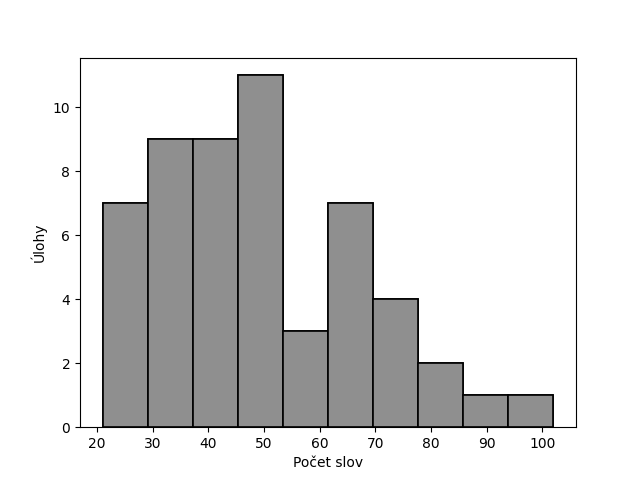
\includegraphics[width=\textwidth]{assets/words.png}
\end{subfigure}
\hfill
\begin{subfigure}[b]{0.32\textwidth}
\centering
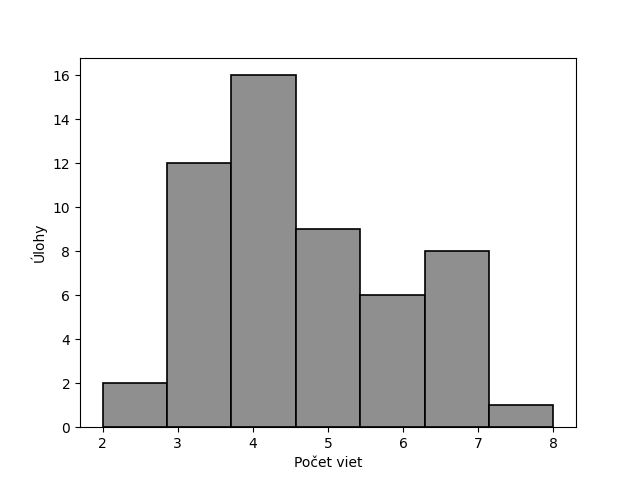
\includegraphics[width=\textwidth]{assets/sentences.png}
\end{subfigure}
\hfill
\begin{subfigure}[b]{0.32\textwidth}
\centering
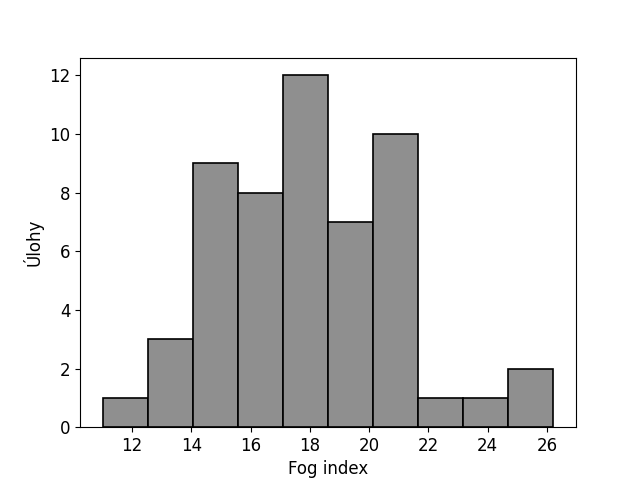
\includegraphics[width=\textwidth]{assets/fog.png}
\end{subfigure}
\hfill
\caption{Kvantifikatívne vlastnosti textu úloh}
\label{fig:text-metrics}
\end{figure}

V prílohe \ref{chapter:appendix-kategorie} sú získané hodnoty v tabuľkách pre všetky znenia cvičení zoskupené po kapitolách. Histogramy (\ref{fig:text-metrics}) poukazujú na to, že priemerný počet slov naprieč zadaniami je $49\; \pm 18$ a teda dominujú kratšie texty v rozmedzí $30$ až $80$ slov. Priemerný počet viet je $4\; \pm 1$ a žiaden text ich nemá viac ako $8$. Fog index sa sústreďuje okolo skóre $18\; \pm 3$, čo značí že texty sú primerane zrozumiteľné pre žiakov stredných škôl. Vo všeobecnosti texty so skóre pod 20 sa pokladajú za veľmi ľahko čitateľné. Do vzorca fog indexu vstupuje počet slov na vetu, ktorých priemer je $10 \pm 2$, a percento ťažkých slov zo všetkých, tých je priemerne $33.9\%\; \pm 8\%$.

Merania fog indexu sme brali výhradne ako doporučenie na úpravu textu, vzhľadom na uspôsobenosť anglickým textom kritériom pre náročné slová a optimálnu dĺžku textu 100 slov. Napiek tomu sme niektoré cvičenia s značne vyšším fog indexom uspôsobili skrátením komplikovaním viet a zamenením náročnejších slov za bežné. Hodnovernejšie posúdenie by poskytlo sémantické kritérium špeciálne pre úlohy, také nám však nie je známe. 

\subsection{Predloha štruktúry úlohy}
Aby podoba znení pôsobila rovnorodým dojmom pridržiavame sa stáleho rozvrhnutia vnútorného usporiadanie textu cvičenia. Zadanie sa začína opisom scenérie prostredia, kde sa dej odohráva. Nasledujú fakty, vzťahy a požiadavky na vstupy uvádzajúce algoritmizovateľnú problémovú situáciu. Úryvok ukončuje najčastejšie explicitné vyjadrenie pokynu v rozkazovacom spôsobe. Pokyn na riešenie nemusí byť priamo vyslovený. Na objasnenie očakávaní techník, ktoré má žiak zvoliť pri riešení, slúži ukážka behu programu. 

Prítomnosť opísaných štruktúrnych prvkov textu dokladáme vybranými úlohami zo zbierky. Tri hlavné časti nazývame skrátene: \textbf{scenéria, problém a pokyn}.

\paragraph{1.5. Hlboká roklina}
\begin{quote}
(\textbf{Scenéria}): \textit{\small ,,Stojíš nad hlbokým údolím za zábradlím a uvažuješ ako odmerať jeho hĺbku. Vtom si spomenieš na svoje vedomosti z fyziky. Zoberieš si do ruky povaľúci sa kameň a pustíš ho priamo do rokliny.''}

(\textbf{Problém}):  \textit{\small Zároveň stlačíš stopky, ktorými zmeriaš čas do dopadu v sekundách. Kameň padá nadol voľným pádom. Stopky zastaviš pri započutí rachotu z nárazu. 
Pri výpočte zanedbáme rýchlosť zvuku, ktorou sa rachot rožšíri až k nám.''}

(\textbf{Pokyn}): Implicitný
\end{quote}

\paragraph{1.8. Kúpalisko}
\begin{quote}
(\textbf{Scenéria}): \textit{\small ,,Začína sa horúca letná sezóna. Prevádzka kúpaliska musí pred otvorením napustiť bazény.''}

(\textbf{Problém}):  \textit{\small Všetky bazény v areáli sú kvádrového tvaru, ktorých rozmery poznáme. Vedúceho kúpaliska zaujíma spotrebovaná voda pre bazén, keď bude napustený pod okraj. Voda nie je zadarmo, preto si chcú pripraviť dosť peňazí, aby za ňu zaplatili.''}

(\textbf{Pokyn}): Implicitný
\end{quote}

\paragraph{2.1. Heslo}
\begin{quote}
(\textbf{Scenéria}): \textit{\small ,,Tvoj dom na strome už vykradlo pár nezvaných návštevníkov. Vymyslel si preto spôsob ako dovoliť návštevu len overeným osobám.''}

(\textbf{Problém}): \textit{\small ,,Tie musia poznať tajné heslo.''}

(\textbf{Pokyn}): \textit{\small ,,Napíš program, ktorý slovne privíta členov a odoženie zlodejov.''}
\end{quote}

\paragraph{2.4. Morský vánok}
\begin{quote}
(\textbf{Scenéria}): \textit{\small ,,Kapitán plachetnice na otvorenom oceáne musí mať vždy prehľad odkiaľ fúka vietor, aby dokormidloval do vytúženého cieľa. Príliš silné závany vetra môžu byť nebezpečné pre posádku. Rozthať polámať lodné sťažne, potrhať plachty, či zaplaviť palubu.''}

(\textbf{Problém}): \textit{\small ,,Cez rádio dostáva plavidlo každý deň správy o predpovedi sily vetra v Beafortovej stupnici. Sila vetra je ňou vyjadrená do dvanástich stupňov od bezvetria až po orkán.''} 

(\textbf{Pokyn}): \textit{\small ,,Napíš program, ktorý kapitánu vysvetlí stupeň vetra. Podľa stupnice určíme jeho pomenovanie, rýchlosti v námorných uzloch a očakávateľnej výšky vĺn.''}
\end{quote}

\paragraph{5.5. Výskyt písmen}
\begin{quote}
(\textbf{Scenéria}): \textit{\small ,,Dlho do noci čítaš časopisy o umelej inteligencii a fascinuje ťa jej schopnosť rozprávať sa s človekom.''} 

(\textbf{Problém}): \textit{\small ,,Na vytvorenie viet na danú tému potrebuje mať prehľad o percentuálnom výskyte hlások v texte.''}

(\textbf{Pokyn}): \textit{\small ,,Spočítaj a vypíš zoznam početnosti písmen v reťazci.''}
\end{quote}

\paragraph{7.1. Vraky}
\begin{quote}
(\textbf{Scenéria}): \textit{\small ,,V šírich hlbinách Atlantiku sa stále ukrýka nepreberné bohatstvo vo vrakoch potopených lodí. V tejto minihre odkryješ tajomstvo skrývajúce sa pod hladinou.''} 

(\textbf{Problém}): \textit{\small ,,Cieľom je nájsť vrak parníka na náhodnej pozícii.''} 

(\textbf{Pokyn}): \textit{\small ,,Do programu napíš funkciu vzdialenost(x, y), ktorá na základe zadaných súradníc vypočíta ako ďaleko si od vraku.''}
\end{quote}

 
Písomný prejav má tvar 2. osoby jednotného čísla, čím si kladieme predpoklad, že zlepšíme zrorumiteľnosť, keď sa priblížime reči rovesníkov. Uľahčenie v chápaní komunikačného zámeru dosiahnutý pravideľnosťou, umožujeme pridať na inferečnej zložitosti. Namiesto žiakovho sústredenia sa na povrchovú orientáciu v texte ponechávame priestor na vyvodzovanie súvislostí, čím podporujeme čítanie s porozumením. 

Grafická úprava úlohy je taktiež ujednotená a sa skladá z nadpisu, textu zadania, ukážka vzorového súboru ak je prítomná, vstupov a výstupov programu. Nadpis úlohy obsahuje číselné označeníe kapitoly, poradia úlohy vnútri kapitoly a jej názov v podobe slovného spojenia.
Vstupy a výstupy programu sú orámované v oblasti so šedým pozadím, písmo je neproporciálne, a premenlivé údaje závislé od vstupov sú zastúpené prázdnymi obdĺžnikmi. Na ilustáciu modelového spustenia programu môžu byť do obdĺžnikov niekedy vpísané konkrétne hodnoty.


\subsection{Didaktické funkcie úloh}
Graduálne stupňovanie náročnosti úloh do troch úrovní, rovnomerné zastúpenie náplňania rozličných didaktických funkcií a zapojenia viacerých kognitívných úrovní overíme zaklasifikovaním úloh. Príloha \ref{chapter:appendix-kategorie} zachytáva zaradenie samotných zadaní do systému úloh. Tému, podtému a element sú prevažne predurčené názvom kapitoly, preto tie nešpecifikujeme. 

Určenie didaktických funkcií úlohy je do značnej miery subjektívne, preto na odôvodnenie našich rozhodnutí ponúkame osobitnú interpretáciu kategorizácie. Motivačná funkcia ..

%TODO opíš didaktické funckie
Zoradenie úloh je podľa náročnosti, do tém a podtém podľa toho ktorý najzložitejší pojem alebo postup sa v nich vyskytuje

Tabuľky na didaktické funkcie, kognitívnu úroveň
zaradie úloh do kategórii závisí od ich poradia v zbierke


Pozorovanie ako to žiaci zvládali




